%----------------------------------------------------------------------------------------
%   Доорх хэсгийг өөрчлөх шаардлагагүй
%----------------------------------------------------------------------------------------
%!TEX TS-program = xelatex
%!TEX encoding = UTF-8 Unicode
\documentclass[12pt,A4]{report}

\usepackage{fontspec,xltxtra,xunicode}
\setmainfont[Ligatures=TeX]{Times New Roman}
\setsansfont{Arial}

% \usepackage[utf8x]{inputenc}
% \usepackage[mongolian]{babel}
%\usepackage{natbib}
\usepackage{geometry}
%\usepackage{fancyheadings} fancyheadings is obsolete: replaced by fancyhdr. JL
\usepackage{fancyhdr}
\usepackage{float}
\usepackage{afterpage}
\usepackage{graphicx}
\usepackage{amsmath,amssymb,amsbsy}
\usepackage{dcolumn,array}
\usepackage{tocloft}
\usepackage{dics}
\usepackage{nomencl}
\usepackage{upgreek}
\newcommand{\argmin}{\arg\!\min}
\usepackage{mathtools}
\usepackage[hidelinks]{hyperref}
\usepackage{tabularx}

\usepackage{algorithm}
\usepackage{algpseudocode}

\usepackage{listings}
\DeclarePairedDelimiter\abs{\lvert}{\rvert}%
\makeatletter
\usepackage{caption}
\captionsetup[table]{belowskip=0.5pt}
\usepackage{subfiles}

\usepackage{listings}
\renewcommand{\lstlistingname}{Код}
\renewcommand{\lstlistlistingname}{\lstlistingname ын жагсаалт}

\usepackage{color}
\definecolor{codegreen}{rgb}{0,0.6,0}
\definecolor{codegray}{rgb}{0.5,0.5,0.5}
\definecolor{codepurple}{rgb}{0.58,0,0.82}
\definecolor{backcolour}{rgb}{0.99,0.99,0.99}
 
\lstdefinestyle{mystyle}{
    basicstyle=\ttfamily\small,
    backgroundcolor=\color{backcolour},   
    commentstyle=\color{codegreen},
    keywordstyle=\color{magenta},
    numberstyle=\tiny\color{codegray},
    stringstyle=\color{codepurple},
    %basicstyle=\footnotesize,
    breakatwhitespace=false,         
    breaklines=true,                 
    captionpos=b,                    
    keepspaces=false,                 
    numbers=left,                    
    numbersep=10pt,                  
    showspaces=false,                
    showstringspaces=true,
    showtabs=false,                  
    tabsize=2
}
 
\lstset{style=mystyle, label=DescriptiveLabel} 

\let\oldabs\abs
\def\abs{\@ifstar{\oldabs}{\oldabs*}}
\makenomenclature
\begin{document}


%----------------------------------------------------------------------------------------
%   Өөрийн мэдээллээ оруулах хэсэг
%----------------------------------------------------------------------------------------

% Дипломийн ажлын сэдэв
\title{АЖИЛ ОЛГОГЧДЫН ӨГӨГДЛИЙН АНАЛИЗ СИСТЕМ ДЭЭР СУУРИЛСАН ЧАТ БОТ}
% Дипломын ажлын англи нэр
\titleEng{Chat bot based on sytem analysis of employers' data}
% Өөрийн овог нэрийг бүтнээр нь бичнэ
\author{Анужингийн Сайнзолбоо}
% Өөрийн овгийн эхний үсэг нэрээ бичнэ
\authorShort{А.Сайнзолбоо}
% Удирдагчийн зэрэг цол овгийн эхний үсэг нэр
\supervisor{Б.Хуягбаатар доктор (Ph.D.)}
% Хамтарсан удирдагчийн зэрэг цол овгийн эхний үсэг нэр

% СиСи дугаар 
\sisiId{18B1NUM1762}
% Их сургуулийн нэр
\university{МОНГОЛ УЛСЫН ИХ СУРГУУЛЬ}
% Бүрэлдэхүүн сургуулийн нэр
\faculty{ХЭРЭГЛЭЭНИЙ ШИНЖЛЭХ УХААН, ИНЖЕНЕРЧЛЭЛИЙН СУРГУУЛЬ}
% Тэнхимийн нэр
\department{МЭДЭЭЛЭЛ, КОМПЬЮТЕРИЙН УХААНЫ ТЭНХИМ}
% Зэргийн нэр
\degreeName{Бакалаврын судалгааны ажил}
% Суралцаж буй хөтөлбөрийн нэр
\programeName{Мэдээллийн технологи (D061303)}
% Хэвлэгдсэн газар
\cityName{Улаанбаатар}
% Хэвлэгдсэн огноо
\gradyear{2022 оны 03 сар}


%----------------------------------------------------------------------------------------
%   Доорх хэсгийг өөрчлөх шаардлагагүй
%----------------------------------------------------------------------------------------
%----------------------Нүүр хуудастай хамаатай зүйлс----------------------------
\pagenumbering{roman}
\makefrontpage
\maketitle

\doublespace

% Гарчгийг автоматаар оруулна
\setcounter{tocdepth}{1}
\tableofcontents

% Зургийн жагсаалтыг автоматаар оруулна
\listoffigures

% This puts the word "Page" right justified above everything else.
\newpage
%% \addtocontents{lof}{Зураг~\hfill Хуудас \par}
\newpage
%% \addtocontents{lot}{Хүснэгт~\hfill Хуудас \par}

\renewcommand{\cftlabel}{Зураг}


\doublespace
\pagenumbering{arabic}


\begin{abstract}

<<<<<<< HEAD
=======
Мэдээллийн технологи эрчимтэй хөгжиж буй өнөөгийн нийгэмд байгууллага үйл ажиллагаа явуулж эхэлсэн цагаасаа эхлэн өгөгдлийг үйлдвэрлэсээр байдаг. Тэдгээр өгөгдлийг байнга хадгалах нь өгөгдлийн сангийн нөөцөд хортой байдаг тул өгөгдөлд шинжилгээ хийх
\newline
\quad \quad \textbf{Зорилго} React болон Next.js технологийн талаар судалж, компанийн хөгжүүлэлтийн арга барилтай танилцахReact болон Next.js технологийн талаар судалж, компанийн хөгжүүлэлтийн арга барилтай танилцах
React болон Next.js технологийн талаар судалж, компанийн хөгжүүлэлтийн арга барилтай танилцах
 
 
\quad \quad \textbf{Зорилт} Удирдагчийн зааварчилгааны дагуу алхам алхмаар судалгаа хийж өгсөн шаардлагын хүрээнд хэрэгжүүлэлт хийх
>>>>>>> 7adbb2fbaa485c537ecc752be489a676d2c3f2ae
\end{abstract}


\addcontentsline{toc}{part}{БҮЛГҮҮД}
\chapter{Сэдвийн танилцуулга}
\subfile{chapters/introduction}

\chapter{Системийн судалгаа}
\subfile{chapters/research.tex}

\chapter{Системийн шинжилгээ}
\subfile{chapters/analysis.tex}

\chapter{Системийн зохиомж}
\subfile{chapters/design.tex}

\chapter{Хэрэгжүүлэлт, үр дүн}
\subfile{chapters/implement.tex}

\addcontentsline{toc}{part}{ДҮГНЭЛТ}

\conclusion{Дүгнэлт}
\quad Бакалаврын судалгааны ажлаар ``Ажил олгогчдын өгөгдлийн анализ систем дээр суурилсан чатбот'' сэдвийн дагуу хөгжүүлэлтийг эхлүүлсэн бөгөөд уг судалгааны ажилд холбогдох онолын судалгаа, ашиглаж буй технологи, түүнийг илүү онолын мэдлэг болон системийн хөгжүүлэлтийн хэсгээс дэлгэрэнгүй тайлбарласан болно.

Системийг хөгжүүлэхдээ уламжлалт холбоост өгөгдлийн сан(relational database) санг ашиглаж нийт өгөгдлийг zangia.mn-ээс цуглуулан ашиглав. Системийг Microsoft Azure платформын Bot Framework-д тулгуурлан javascript хэл дээр хөгжүүлсэн бөгөөд цаашид хэрэглэгчдэд хүргэхэд олон төрлийн сувгийг ашиглан хөгжүүлэх боломжтой.

\singlespace
\addcontentsline{toc}{part}{НОМ ЗҮЙ}
\begin{thebibliography}{99}
	\bibitem{chatbotsystem}
	Чатбот системийн тухай
	\\\url{https://www.engati.com/blog/types-of-chatbots-and-their-applications}
\end{thebibliography}



%----------------------------------------------------------------------------------------
%   Хавсралтууд эндээс эхэлнэ
%----------------------------------------------------------------------------------------
\appendix
\addcontentsline{toc}{part}{ХАВСРАЛТ}

% Хавсралтын нэр. Хавсралт гэдэг үг агуулахгүй
\chapter{Үечилсэн төлөвлөгөө}
\begin{figure}[h]
	\centering
	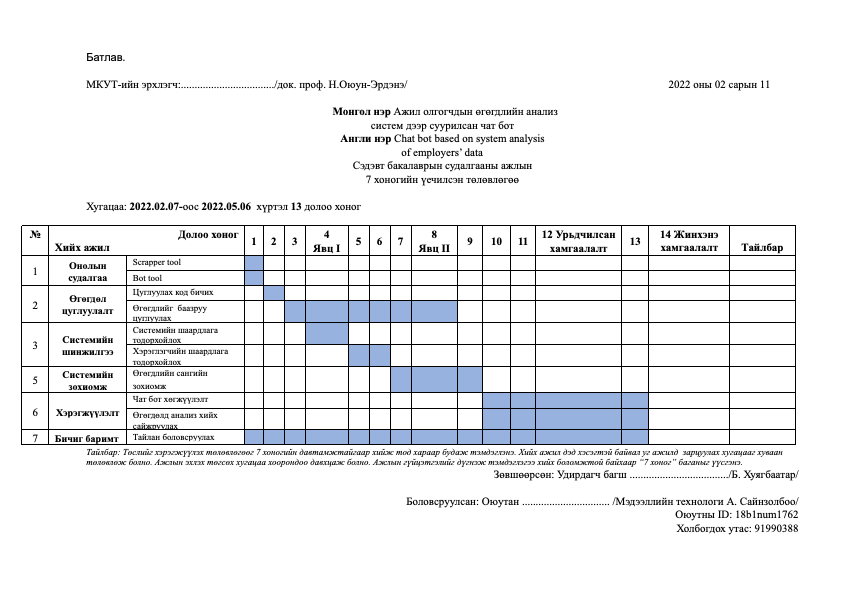
\includegraphics[width=16.5cm, angle=90]{images/plan.png}
	\caption{Бакалаврын судалгааны ажлын үечилсэн төлөвлөгөө}
	\label{fig:plan01}
\end{figure}
% Хавсралтын нэр. Хавсралт гэдэг үг агуулахгүй
\chapter{Кодын хэрэгжүүлэлт}

\section{Өгөгдөл цугуулалт}
Өгөгдөл цуглуулах програм нь дараах бүтэцтэй байх бөгөөд assets доторх кодууд нь үндсэн кодыг ажлуулахад туслах функцууд байна.
\begin{figure}[h]
	\centering
	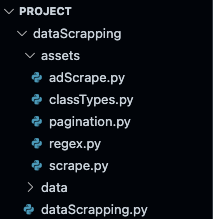
\includegraphics[width=5cm]{images/folderStructure.png}
	\caption{Фолдерийн бүтэц}
	\label{fig:plan01}
\end{figure}
\subsection{Үндсэн өгөгдлийг цуглуулах эх код}
\lstinputlisting[language=Python, caption=Бүх өгөгдлийг цуглуулах - dataScrapping.py]{code/dataScrapping.py}
\subsection{Нэг зарын шаардлагатай бүх мэдээллийг цуглуулах код}
\lstinputlisting[language=Python, caption=Нэг зарын өгөгдлийг цуглуулах - adScrape.py]{code/adScrape.py}
\subsection{Цуглуулах өгөгдлийн төрөл}
\lstinputlisting[language=Python, caption=Өгөгдлийн төрөл - classTypes.py]{code/classTypes.py}
\subsection{Url хаягийн html-ийг авах функц}
\lstinputlisting[language=Python, caption=Scrape хийх функц - classTypes.py]{code/classTypes.py}
% \begin{lstlisting}[language=Python]{../hello.c}

\end{document}